\clearpage
\subsection{รับค่าจากมอเตอร์แล้วมาแสดงผลใน RViz}

\begin{figure}[!ht]
    \centering
    \begin{subfigure}[b]{0.45\textwidth}
        \centering
        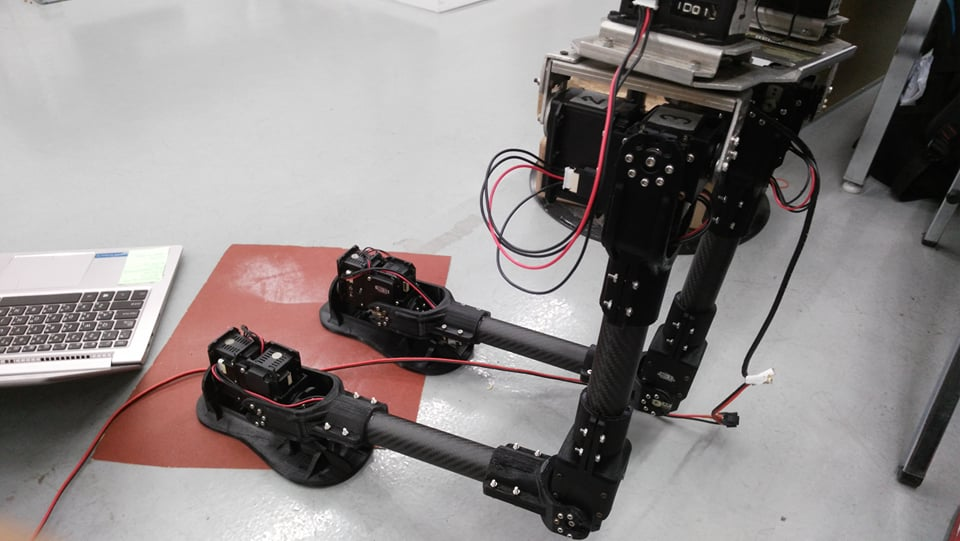
\includegraphics[width=\textwidth]{chapter4/images/robot_2_rviz1.jpg}
        \caption{หุ่นยนต์ตัวจริง}
    \end{subfigure}
    \hfill
    \begin{subfigure}[b]{0.45\textwidth}
        \centering
        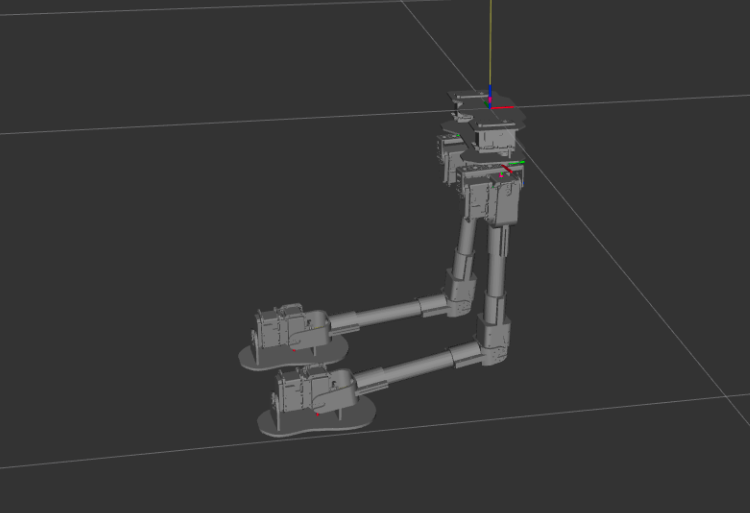
\includegraphics[width=\textwidth]{chapter4/images/robot_2_rviz1.png}
        \caption{หุ่นยนต์ใน RViz}
    \end{subfigure}
    \caption{การแสดงผลท่าทาง 1}
	\label{fig:robot_2_rviz1}
\end{figure}

\begin{figure}[!ht]
    \centering
    \begin{subfigure}[b]{0.45\textwidth}
        \centering
        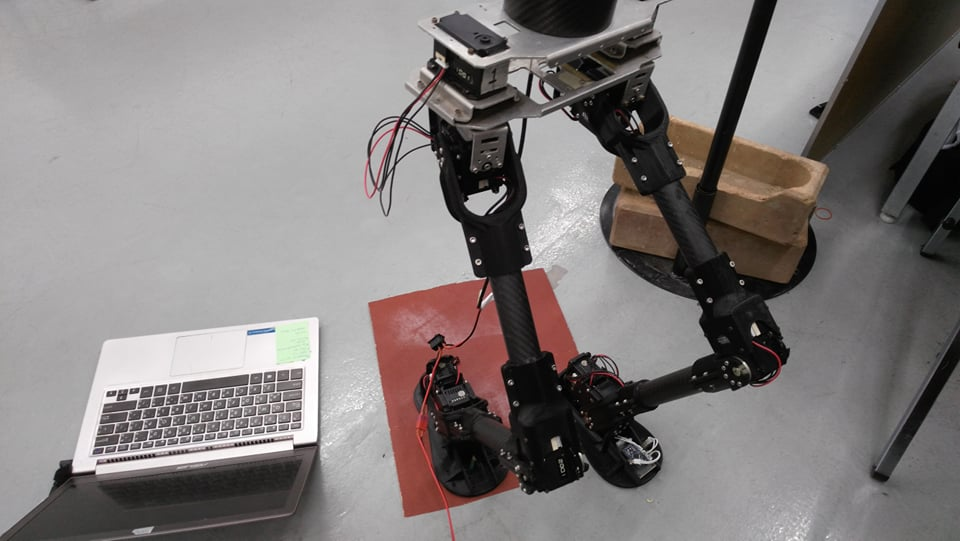
\includegraphics[width=\textwidth]{chapter4/images/robot_2_rviz2.jpg}
        \caption{หุ่นยนต์ตัวจริง}
    \end{subfigure}
    \hfill
    \begin{subfigure}[b]{0.35\textwidth}
        \centering
        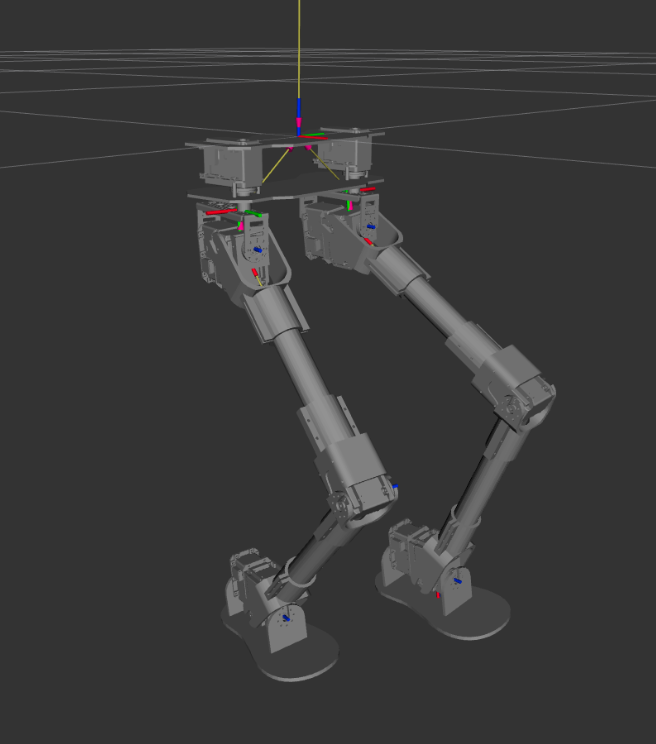
\includegraphics[width=\textwidth]{chapter4/images/robot_2_rviz2.png}
        \caption{หุ่นยนต์ใน RViz}
    \end{subfigure}
    \caption{การแสดงผลท่าทาง 2}
	\label{fig:robot_2_rviz2}
\end{figure}

\begin{figure}[!ht]
    \centering
    \begin{subfigure}[b]{0.45\textwidth}
        \centering
        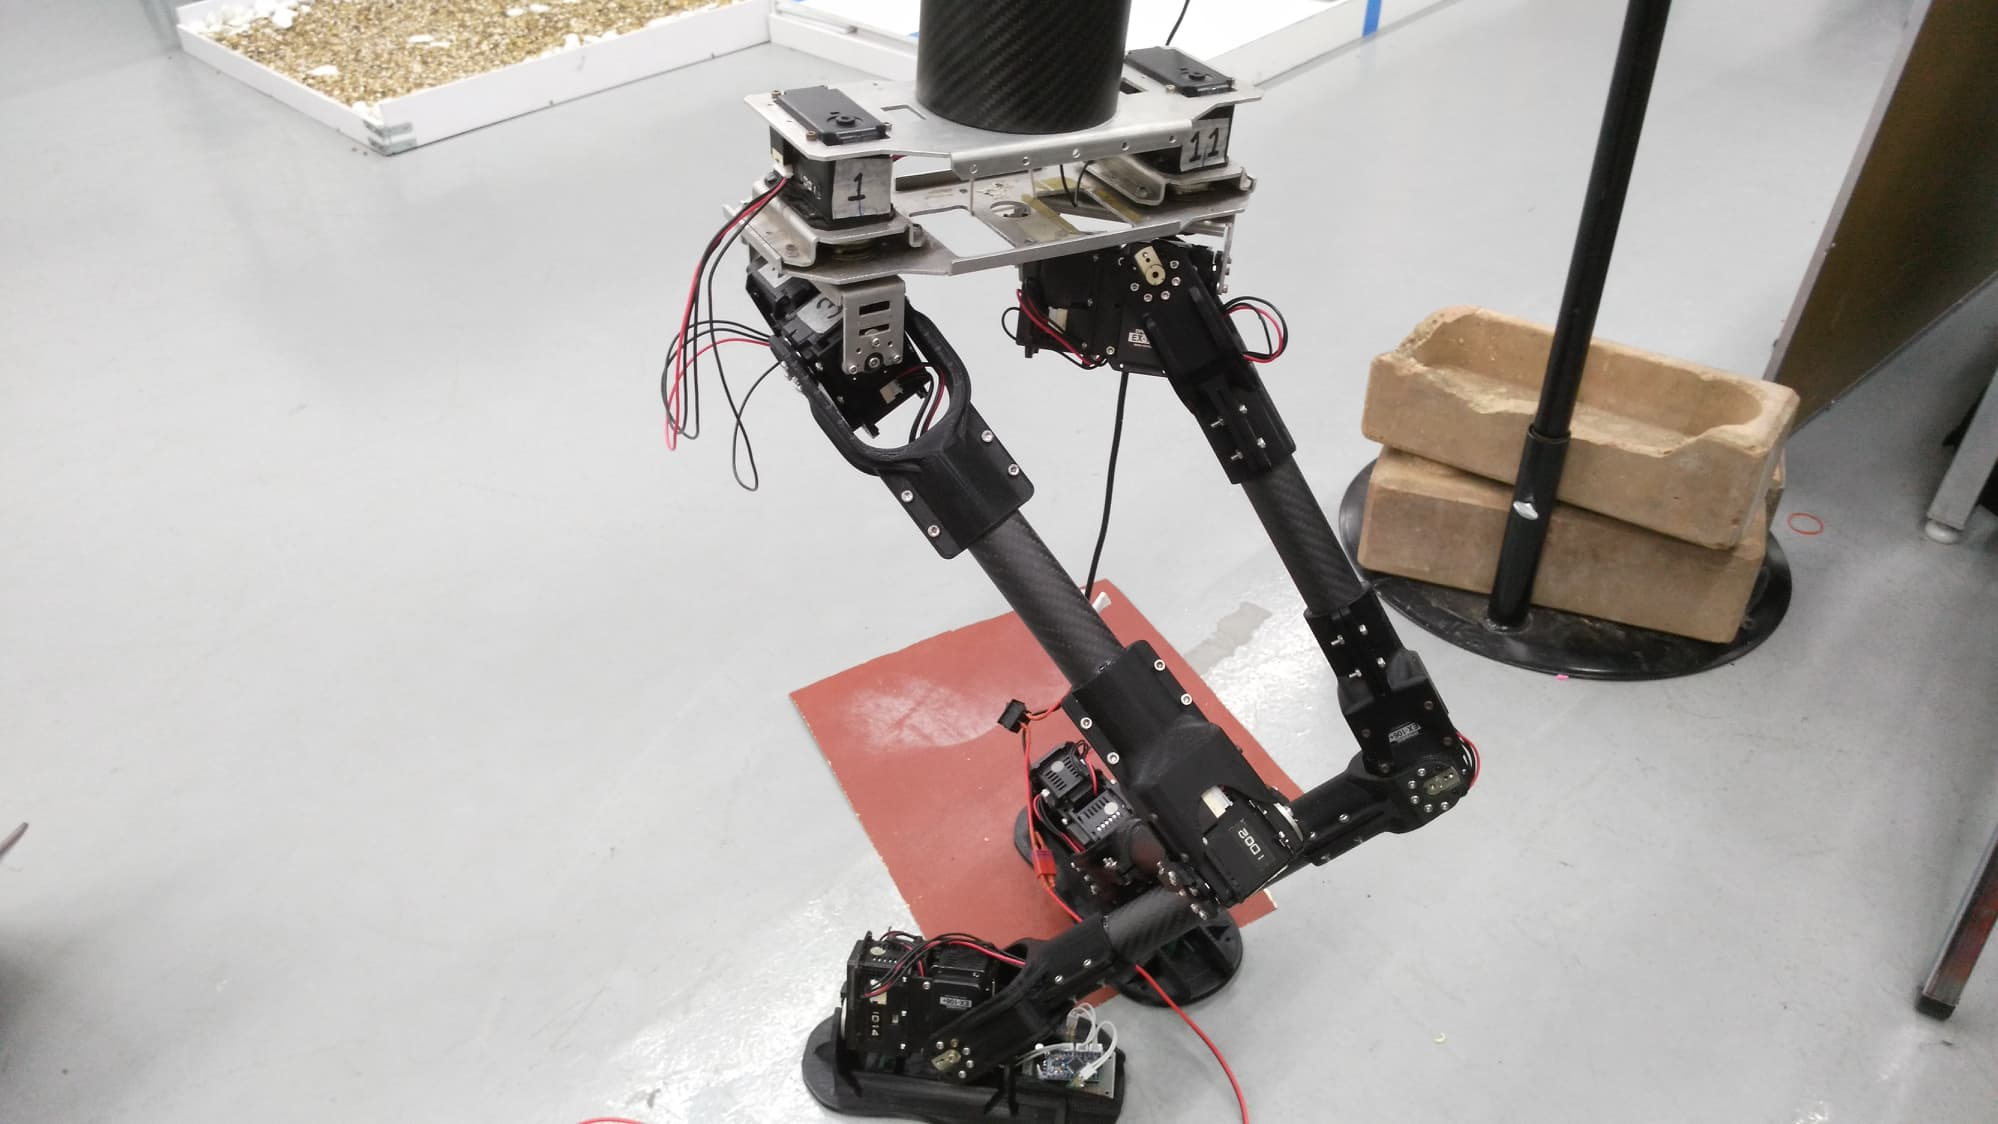
\includegraphics[width=\textwidth]{chapter4/images/robot_2_rviz3.jpg}
        \caption{หุ่นยนต์ตัวจริง}
    \end{subfigure}
    \hfill
    \begin{subfigure}[b]{0.35\textwidth}
        \centering
        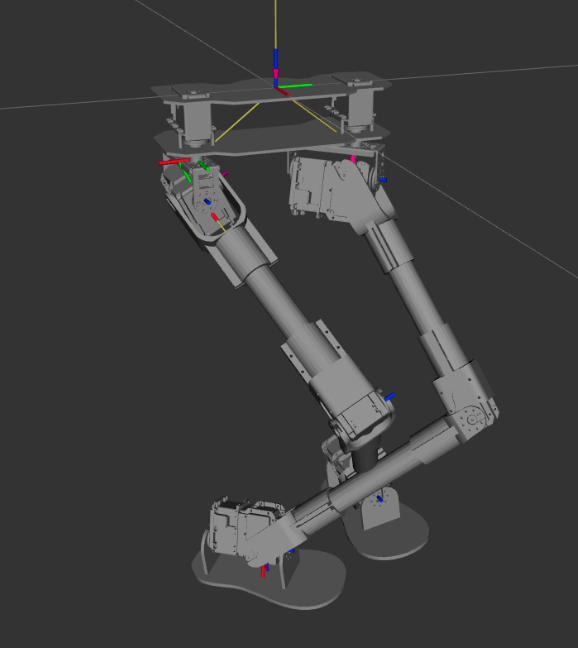
\includegraphics[width=\textwidth]{chapter4/images/robot_2_rviz3.png}
        \caption{หุ่นยนต์ใน RViz}
    \end{subfigure}
    \caption{การแสดงผลท่าทาง 3}
	\label{fig:robot_2_rviz3}
\end{figure}


\clearpage
\subsection{Simulation Gazebo}
ต้องติดตั้ง package ต่อไปนี้

% \begin{enumerate}[label=\arabic*, leftmargin=1.5cm]
% 	\item controller_manager\*
%     \item gazebo_ros_control\*
%     \item joint_state_controller
%     \item effort_controller
% \end{enumerate}

\begin{enumerate}[label=\arabic*, leftmargin=1.5cm]
	\item joint\_state\_controller
	\item effort\_controller
	\item controller\_manager*
	\item gazebo\_ros\_control*
\end{enumerate}